% Created 2023-01-12 Πεμ 22:39
% Intended LaTeX compiler: pdflatex
\documentclass[11pt]{article}
\usepackage[utf8]{inputenc}
\usepackage[T1]{fontenc}
\usepackage{graphicx}
\usepackage{longtable}
\usepackage{wrapfig}
\usepackage{rotating}
\usepackage[normalem]{ulem}
\usepackage{amsmath}
\usepackage{amssymb}
\usepackage{capt-of}
\usepackage{hyperref}
\usepackage{booktabs}
\usepackage{import}
\usepackage[LGR, T1]{fontenc}
\usepackage[greek, english]{babel}
\usepackage{alphabeta}
\usepackage{esint}
\usepackage{mathtools}
\usepackage{esdiff}
\usepackage{makeidx}
\usepackage{glossaries}
\usepackage{newfloat}
\usepackage{minted}
\usepackage{chemfig}
\usepackage{svg}
\usepackage[a4paper, margin=3cm]{geometry}
\author{Vidianos Giannitsis}
\date{\today}
\title{Βασικά Κομμάτια της Διεργασίας}
\hypersetup{
 pdfauthor={Vidianos Giannitsis},
 pdftitle={Βασικά Κομμάτια της Διεργασίας},
 pdfkeywords={},
 pdfsubject={},
 pdfcreator={Emacs 28.2 (Org mode 9.5.5)}, 
 pdflang={English}}
\makeatletter
\newcommand{\citeprocitem}[2]{\hyper@linkstart{cite}{citeproc_bib_item_#1}#2\hyper@linkend}
\makeatother

\usepackage[notquote]{hanging}
\begin{document}

\maketitle
\tableofcontents

\renewcommand{\abstractname}{Περίληψη}
\renewcommand{\tablename}{Πίνακας}
\renewcommand{\figurename}{Σχήμα}
\renewcommand\listingscaption{Κώδικας}

\begin{abstract}
Μία συχνή τακτική για την παρουσίαση μεγάλων διεργασιών όπου το συνολικό διάγραμμα ροής που προκύπτει είναι πολύ μεγάλο είναι οι διεργασίες να χωρίζονται σε blocks αριθμημένα με τη λογική 100, 200, 300 κλπ. Καθώς η διεργασία που έχουμε σχεδιάσει για το μάθημα είναι πολύ μεγάλη, θα ακολουθηθεί αυτή η προσέγγιση. Παρακάτω θα αναφερθούν τα blocks στα οποία θα διαμεριστεί η διεργασία χωρίς πολύ εξήγηση για τώρα και έπειτα θα εξηγηθούν επαρκώς για την εργασία.
\end{abstract}

\section{Block 100 - Διαχωρισμός των τριών κομματιών της βιομάζας}
\label{sec:org40a08e8}
Το block αυτό είναι για την βασική διεργασία διαχωρισμού την έκρηξη ατμού και της επακόλουθες διεργασίες διαχωρισμού κυτταρίνης-λιγνίνης. Ως τροφοδοσία έχει νερό για παραγωγή ατμού, πυρηνόξυλο (πρώτη ύλη) και τα υδατικά διαλύματα που απαιτούνται για τις διεργασίες διαχωρισμού. Προιόντα είναι τα τρία βασικά ρεύματα ξυλόζης, κυτταρίνης και λιγνίνης.

\begin{figure}[htbp]
\centering
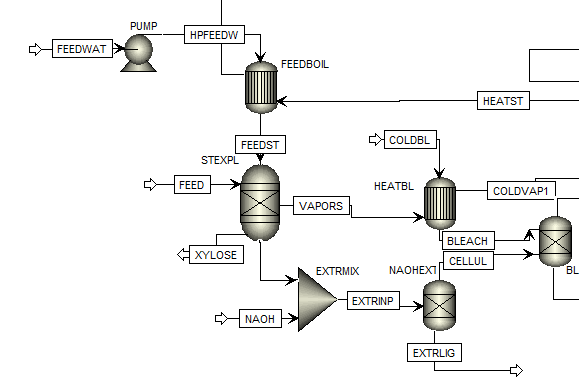
\includegraphics[width=.9\linewidth]{Block_100_-_Steam_Explosion/2023-01-10_18-30-22_screenshot.png}
\caption{Block 100 στο Aspen}
\end{figure}

Σε αυτό περιέχεται μία αντλία για να φέρει το νερό σε πίεση 26 bar, ένας εναλλάκτης που το θερμαίνει για να παράξει τον υπέρθερμο ατμό που χρησιμοποιείται στη διεργασία (ο οποίος λειτουργεί με ατμό υψηλής πίεσης που παρέχει η εγκατάσταση). Ο θάλαμος της έκρηξης ατμού στον οποίο μπαίνει βιομάζα και ατμός και παράγονται, η υδατοδιαλυτή φάση με κυρίως ημικυτταρινικά συστατικά, η οποια θα χρησιμοποιηθεί ως τροφοδοσία του block 600, η στερεή φάση (λιγνίνη και κυτταρίνη), η οποία απαιτεί περαιτέρω διαχωρισμό και η ατμώδης φάση που είναι πρακτικά η απώλεια μάζας κατά την διεργασία. Η διεργασία προσομοιώθηκε σε RYield αντιδραστήρα καθώς είναι γνωστό ποιά είναι τα yields των προιόντων και υπάρχουν χημικές μετατροπές άρα δεν μπορεί να είναι απλό separator. Έπειτα, φαίνονται και οι 2 διεργασίες διαχωρισμού κυτταρίνης-λιγνίνης.

Η πρώτη είναι μία εκχύλιση υγρού-στερεού με υδατικό διάλυμα NaOH για τον κύριο διαχωρισμό και για να διώξουμε όλη την ποσότητα της λιγνίνης και όχι μόνο αυτήν που φεύγει με την εκχύλιση υπάρχει και ένα bleacher το οποίο χρησιμοποιεί NaClO για να διώξει πλήρως την λιγνίνη. Ο bleacher λειτουργεί σε θερμοκρασία υψηλότερη από αυτή του περιβάλλοντος για αυτό απαιτείται ένας εναλλάκτης για την θέρμανση του ρεύματος. Και οι δύο έχουν προσομοιωθεί ως απλά separators καθώς θα ήταν πολύ δύσκολο να εισαχθούν στο Aspen τα κατάλληλα θερμοφυσικά δεδομένα για να προσομοιωθούν με ακρίβεια οι διεργασίες.

Ένα πρόβλημα που υπάρχει είναι ότι κατά την ανάμιξη του στερεού ρεύματος με το υδατικό διάλυμα NaOH, το διάλυμα θερμαίνεται και εξατμίζεται, με αποτέλεσμα να μην υπάρχει εκχύλιση υγρού-στερεού. Αυτή είναι μία παράλειψη της διεργασίας η οποία δεν έχει διορθωθεί λόγω χρόνου.

\section{Block 200 - Παραγωγή Γλυκόζης}
\label{sec:org6d7da72}
Στο block αυτό θεωρείται ως τροφοδοσία η καθαρή κυτταρίνη του block 100 και νερό το οποίο απαιτείται για την υδρόλυση της κυτταρίνης. Προιόν της διεργασίας είναι η γλυκόζη που θα τροφοδοτηθεί στον βιοαντιδραστήρα παραγωγής γλυκερόλης (block 400).

\begin{figure}[htbp]
\centering
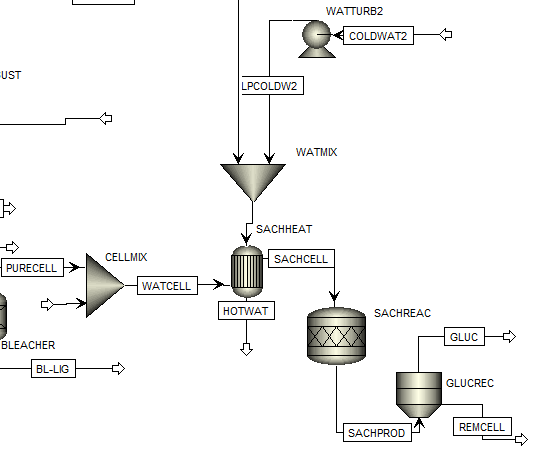
\includegraphics[width=.9\linewidth]{Block_200_-_Παραγωγή_Γλυκόζης/2023-01-10_18-39-54_screenshot.png}
\caption{Block 200 στο Aspen}
\end{figure}


Αρχικά φαίνεται ένα mixer που αναμιγνύει κυτταρίνη με νερό. Έπειτα, υπάρχει ένας εναλλάκτης που ψύχει το ρεύμα αυτό για να φτάσει στη βέλτιστη θερμοκρασία λειτουργίας των κυτταρινάσων (50 \(^oC\)). Όπως αναφέρθηκε στο παραπάνω block, η ψύξη θα έπρεπε να γίνεται στην έξοδο του steam explosion και όχι εδώ, αλλά για τώρα, γίνεται εδώ. Έπειτα, ακολουθεί ο αντιδραστήρας της ενζυμικής υδρόλυσης ή σακχαροποίησης της κυτταρίνης. Καθώς ο αντιδραστήρας αυτός δεν είναι βασικός για την διεργασία και η ολοκληρωμένη ανάλυση του είναι αρκετά περίπλοκη, έχει προσομοιωθεί ως RStoic που πραγματοποιεί την υδρόλυση μίας δομικής μονάδας κυτταρίνης σε γλυκόζη, ορίζοντας ως μετατροπή το ποσοστό κυτταρίνης που γίνεται γλυκόζη. Βέβαια, έτσι δεν καταναλώνεται όλη η κυτταρίνη που μπαίνει στον αντιδραστήρα το οποίο είναι ανακρίβεια λόγω της απλοποιημένης προσέγγισης. Για αυτό υπάρχει ένα decanter το οποίο έχει ως σκοπό τον διαχωρισμό του στερεού από το υδατικό διάλυμα γλυκόζης.

\section{Block 300 - Λέβητας Καύσης Λιγνίνης}
\label{sec:org8160463}
To block αυτό έχει την προσομοίωση του λέβητα που χρησιμοποιείται για την καύση της λιγνίνης. Η λιγνίνη καίγεται και από τα καυσαέρια της παράγεται ατμός υψηλής πίεσης τον οποίο μπορούμε να εκμεταλλευτούμε σε άλλα σημεία της εγκατάστασης. Νερό αντλείται από χαμηλή πίεση μέχρι τα 40 bar η οποία είναι η πίεση λειτουργίας του λέβητα αυτού. Προιόν του block 300 είναι ο ατμός υψηλής πίεσης που είναι αρκετά χρήσιμος για την εγκατάσταση.

\begin{figure}[htbp]
\centering
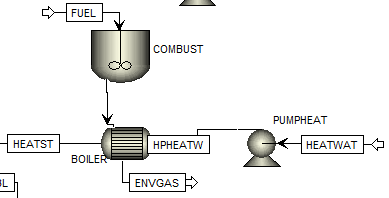
\includegraphics[width=.9\linewidth]{Block_300_-_Λέβητας_Καύσης_Λιγνίνης/2023-01-10_18-51-18_screenshot.png}
\caption{Block 300 στο Aspen}
\end{figure}

Για την προσομοίωση έχει μπει αρχικά ένας καυστήρας λιγνίνης ο οποίος τροφοδοτείται με μίγμα στερεού καυσίμου και αέρα και το καίει. Με βάση την βιβλιογραφία, έχει βρεθεί η θερμογόνος δύναμη του καυσίμου και με ένα ισοζύγιο ενέργειας μπορεί να οριστεί η θερμοκρασία λειτουργίας του λέβητα από την θερμοκρασία των καυσαερίων. Τα καυσαέρια αυτά θερμαίνουν νερό το οποίο γίνεται ατμός υψηλής πίεσης. Ο ατμός υψηλής πίεσης έχει 2 βασικές λειτουργίες σε μία εγκατάσταση. Ηλεκτροπαραγωγή σε μία διάταξη όπως τα κύκλα Rankine και χρήση ως θερμαντικό μέσο. Στην παρούσα φάση χρησιμοποιείται μόνο ως θερμαντικό μέσο για την παραγωγή του ατμού στο Steam explosion, αλλά η προσομοίωση μπορεί να επεκταθεί και για άλλα πράγματα. Επίσης, αν θέλουμε να αυξήσουμε απόδοσης της εστίας καύσης, μπορούμε να χρησιμοποιήσουμε ένα συνδυασμένο κύκλο ατμού-αερίου το οποίο παράγει ατμό ως θερμαντικό μέσο αλλά παράγει και ηλεκτρική ενέργεια από την περίσσεια θερμική ενέργεια των καυσαερίων.

\section{Block 400 - Παραγωγή Γλυκερόλης}
\label{sec:org5a9c9e7}
Στο block αυτό φαίνεται ο βιοαντιδραστήρας του μικροοργανισμού C. glycerinogenes ο οποίος χρησιμοποιείται για την παραγωγή γλυκερόλης. Ως τροφοδοσία χρησιμοποιείται ένα μίγμα υδατικού διαλύματος γλυκόζης μαζί με ουρία (πηγή αζώτου) και επαρκές οξυγόνο για την αερόβια καλλιέργεια. Επίσης στο feed υπάρχει και μικρή ποσότητα βιομάζας για να ξεκινήσει η αντίδραση. Το προίον του αντιδραστήρα θερμαίνεται για να ανακτηθεί η καθαρή γλυκερόλη (block 500) αλλά ως πρώτη βαθμίδα θέρμανσης χρησιμοποιείται η καθαρή γλυκερόλη (προιόν). Έτσι, εκμεταλλευόμαστε την θερμική της ενέργεια και την αποθηκεύουμε σε χαμηλή θερμοκρασία.

\begin{figure}[htbp]
\centering
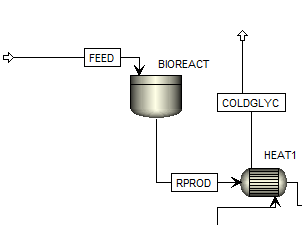
\includegraphics[width=.9\linewidth]{Block_400_-_Παραγωγή_Γλυκερόλης/2023-01-10_19-01-02_screenshot.png}
\caption{Block 400 στο Aspen}
\end{figure}

Ο βιοαντιδραστήρας έχει προσομοιωθεί ως batch αντιδραστήρας. Παρόλο τη μεγάλη κλίμακα στην οποία λειτουργεί το εργοστάσιο, οι βιοαντιδραστήρες γενικά προτιμάται να είναι σε batch λειτουργία επειδή έτσι υπάρχει το flexibility να καθαρίζεται ο αντιδραστήρας συχνά και να μην επιμολύνεται, κάτι που θα προκαλούσε σημαντικά προβλήματα. Παρόλο της χαμηλότερης του απόδοσης από ότι ένας συνεχούς ροής, το γεγονός ότι θα πρέπει η μονάδα να σταματήσει τελειώς για να καθαριστεί σε εκείνη την περίπτωση είναι ένα σημαντικό μειονέκτημα. Αυτό που λείπει από το block αυτό είναι ότι η τροφοδοσία του προκύπτει από το block 200 (γλυκόζη) και δεν έχει προστεθεί ο mixer που θα κάνει την ανάμιξη της γλυκόζης με τα υπόλοιπα απαραίτητα στοιχεία του αντιδραστήρα αυτού.

\section{Block 500 - Καθαρισμός Γλυκερόλης}
\label{sec:org0dd7763}
Το block αυτό είναι για τον διαχωρισμό των προιόντων του βιοαντιδραστήρα και την ανάκτηση της καθαρής εμπορεύσιμης γλυκερόλης. Τροφοδοσία του είναι το προιόν του block 400, δηλαδή τα προιόντα του βιοαντιδραστήρα μετά την πρώτη βαθμίδα θέρμανσης από την γλυκερόλη. Προιόν της διεργασίας είναι η καθαρή γλυκερόλη και δύο υδατικά κλάσματα τα οποία χρησιμοποιούνται για την θέρμανση.

\begin{figure}[htbp]
\centering
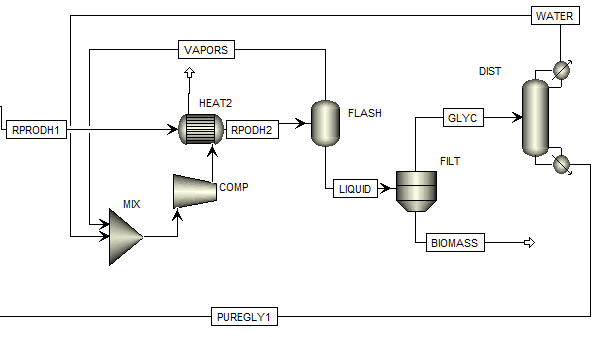
\includegraphics[width=.9\linewidth]{Block_500_-_Καθαρισμός_Γλυκερόλης/2023-01-10_19-09-31_screenshot.png}
\caption{Block 500 στο Aspen}
\end{figure}

Οι διαχωρισμοί που απαιτούνται είναι 3. Αρχικά γίνεται ένα flash στα προιόντα για να διώξουμε όλα τα πτητικά συστατικά. Μετά, μία διήθηση για να ξεχωρίσουμε την στερεή βιομάζα από την γλυκερόλη και έπειτα μία κλασματική απόσταξη για τον τελικό καθαρισμό της γλυκερόλης. Όσο υψηλότερη η θερμοκρασία του flash, τόσο περισσότερο νερό φεύγει μαζί με τα πτητικά συστατικά, άρα τόσο πιό εύκολη η απόσταξη για να πετύχουμε καθαρότητα 0.999. Όμως, όσο αυξάνεται η θερμοκρασία του flash, τόσο περισσότερη γλυκερόλη χάνεται στο flash. Χρησιμοποιήθηκε εν τέλει η θερμοκρασία 140 \(^oC\) η οποία είναι ένα καλό σημείο όπου είναι εύκολη η απόσταξη και χάνεται περίπου το \(10 \%\) της συνολικής γλυκερόλης. Οι ατμοί του flash σε αυτήν την θερμοκρασία, οι οποίοι είναι κατά βάση υδατικοί μπορούν να χρησιμοποιηθούν για την θέρμανση των προιόντων ώστε να τροφοδοτηθούν στο flash. Μαζί με αυτούς χρησιμοποιείται και το νερό που προκύπτει ως απόσταγμα της αποστακτικής στήλης. Για να επαρκούν, πρέπει να έχουν λίγο υψηλότερη πίεση από ότι το ρεύμα που θερμαίνουν, για αυτό υπάρχει και ένας αεροσυμπιεστής ο οποίος έχει ως σκοπό της αύξηση της πίεσης των υδατικών ρευμάτων αυτών.

\section{Block 600 - Παραγωγή Κυκλοπεντανόνης με την Φουρφουράλη ως Ενδιάμεσο}
\label{sec:org86d7d93}
Το block αυτό είναι αυτό που αξιοποιεί την ημικυτταρινική φάση της βιομάζας όπως αυτή βγαίνει από το steam explosion στο block 100. Η προσομοίωση έχει γίνει σε πρώτη φάση υποθέτοντας καθαρό ρεύμα ξυλόζης, βέβαια στην πραγματικότητα, το ρεύμα έχει και άλλα συστατικά τα οποία πρέπει να ληφθούν υπόψην. Στο block αυτό παράγεται αρχικά ένα ενδιάμεσο προιόν, η φουρφουράλη, από την ξυλόζη ενώ αυτή οδηγείται σε έναν δεύτερο αντιδραστήρα, όπου με προσθήκη υδρογόνου, η φουρφουράλη μετατρέπεται σε κυκλοπεντανόνη, το τελικό μας προιόν.

\begin{figure}[htbp]
\centering
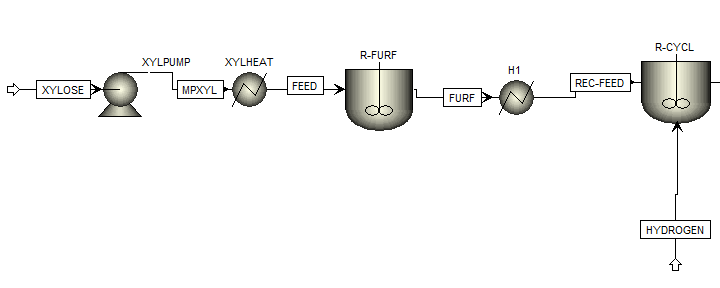
\includegraphics[width=.9\linewidth]{Block_600_-_Παραγωγή_Κυκλοπεντανόνης_με_την_Φουρφουράλη_ως_Ενδιάμεσο/2023-01-10_20-03-27_screenshot.png}
\caption{Block 600 στο Aspen}
\end{figure}

Στο block αυτό παίρνουμε την τροφοδοσία από το block 100 στις συνθήκες του steam explosion, και μέσω μίας αντλίας και ενός εναλλάκτη θερμότητας την φέρνουμε στις συνθήκες του αντιδραστήρα αυτού. Ο αντιδραστήρας παράγει την φουρφουράλη, ένα πολύ χρήσιμο χημικό ενδιάμεσο που παράγεται από την αφυδάτωση της ξυλόζης. Η ξυλόζη δεν μπορεί να μετατραπεί απευθείας σε κυκλοπεντανόνη για αυτό ακολουθείται το μονοπάτι αυτό. Έπειτα, η φουρφουράλη ψύχεται μέχρι τις συνθήκες λειτουργίας του δεύτερου αντιδραστήρα, όπου το ενδιάμεσο αντιδρά σε κυκλοπεντανόνη.

\section{Block 700 - Καθαρισμός της Κυκλοπεντανόνης}
\label{sec:org58734e2}
Το block αυτό έχει ως σκοπό τον καθαρισμό του προιόντος του block 600, δηλαδή του προιόντος του αντιδραστήρα της κυκλοπεντανόνης. Αυτό είναι μίγμα νερού-κυκλοπεντανόνης με μικρή περίσσεια φουρφουράλης και υδρογόνου από την αντίδραση. Προιόν της διεργασίας αυτής είναι η εμπορεύσιμη πλέον κυκλοπεντανόνη υψηλής καθαρότητας.

\begin{figure}[htbp]
\centering
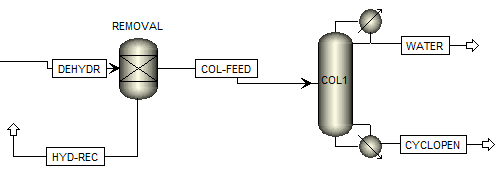
\includegraphics[width=.9\linewidth]{Block_800_-_Καθαρισμός_της_Κυκλοπεντανόνης/2023-01-10_19-56-21_screenshot.png}
\caption{Block 700 στο Aspen}
\end{figure}


Αρχικά, γίνεται ένας διαχωρισμός του υδρογόνου από τα υπόλοιπα συστατικά και έπειτα αυτό ανακυκλώνεται στον αντιδραστήρα. Αυτό έχει γίνει με έναν απλό separator σε πρώτη φάση για να τρέξει η προσομοίωση, αλλά πρακτικά θα γίνει μάλλον με ένα flash στις συνθήκες εξόδου του αντιδραστήρα καθώς στην πίεση λειτουργίας αυτή, όλα τα συστατικά εκτός από το υδρογόνο είναι υγρά. Έπειτα, τα υπόλοιπα οδηγούνται σε μία αποστακτική στήλη η οποία έχει ως σκοπό τον περαιτέρω καθαρισμό της κυκλοπεντανόνης και απομάκρυνση των πτητικών συστατικών (κυρίως νερό). Το προιόν πυθμένα της στήλης είναι κυκλοπεντανόνη υψηλής καθαρότητας.
\end{document}